\subsection{Discussion}
% Mandatory: Create screenshots using Google Earth for each of the scenarios of the collected KML files. The screenshots should include a path that marks the actually walked route. Comment on the results in the report and discuss how GPS errors impacted the results.
% Mandatory: Make a list with the following entries for each scenario: strategy, number of GPS fixes, number of uplink messages, time span, GPS fixes per second, uplink messages per second and comment on them in the report with respect to relevant literature. Discuss what pervasive positioning applications the different strategies are relevant for.

\begin{figure}[h]
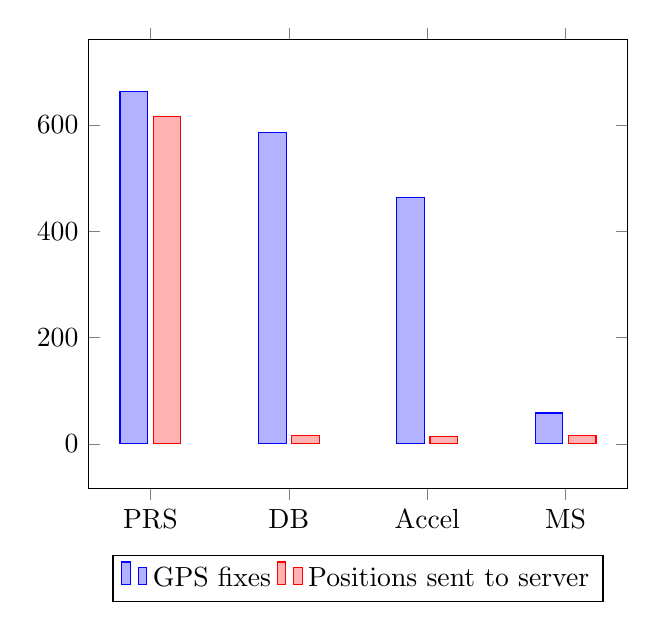
\begin{tikzpicture}
\begin{axis}
	[ybar,
	enlargelimits=0.15,
	legend style={at={(0.5,-0.15)},	anchor=north,legend columns=-1},
	symbolic x coords={PRS, DB, Accel, MS},
	xtick=data]
	
\addplot coordinates
	{(PRS,663) (DB,585) (Accel,463) (MS,58)};
\addplot coordinates
	{(PRS,616) (DB,15) (Accel,14) (MS,16)};

\legend{GPS fixes, Positions sent to server}
\end{axis}
\end{tikzpicture}
\end{figure}

\begin{figure}[h]
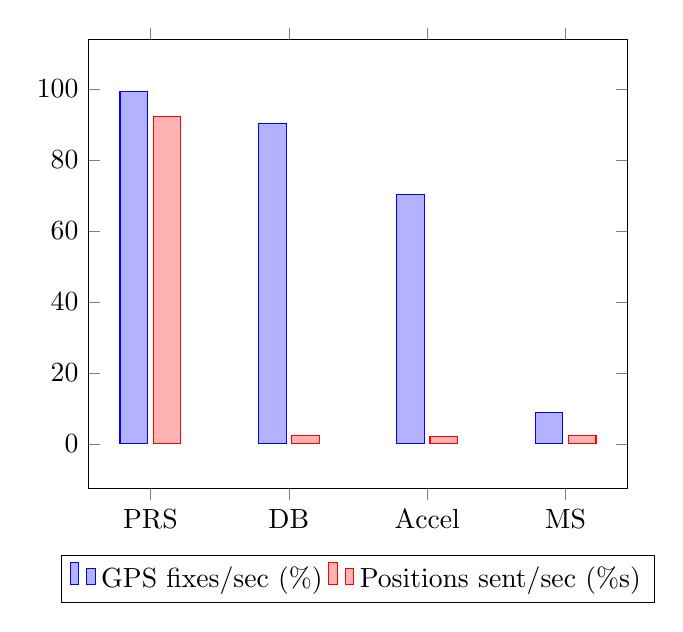
\begin{tikzpicture}
\begin{axis}
	[ybar,
	enlargelimits=0.15,
	legend style={at={(0.5,-0.15)},	anchor=north,legend columns=-1},
	symbolic x coords={PRS, DB, Accel, MS},
	xtick=data]
	
\addplot coordinates
	{(PRS,99.25) (DB,90.28) (Accel,70.15) (MS,8.92)};
\addplot coordinates
	{(PRS,92.22) (DB,2.31) (Accel,2.12) (MS,2.46)};

\legend{GPS fixes/sec (\%), Positions sent/sec (\%s)}
\end{axis}
\end{tikzpicture}
\end{figure}

\begin{table*}[!h]
\begin{tabular}{lrrrrr}

& Number of & Number of & Time span & GPS fixes & Uplink messages \\

& GPS fixes & uplink messages & in seconds & per second & per second \\

\hline

Periodic Reporting Strategy & 663 & 616 & 668 & 99,25 \% & 92,22 \% \\

\hline

Distance-based Reporting Strategy & 585 & 15 & 648 & 90,28 \% & 2,31 \% \\

\hline

DBRS: Accelerometer & 463 & 14 & 660 & 70,15 \% & 2,12 \% \\

\hline

DBRS: Max Speed & 58 & 16 & 650 & 8,92 \% & 2,46 \% \\

\hline

\end{tabular}
\end{table*}